\chapter{Arquitectura de Hardware}\label{ch:tarjeta}

Este trabajo, se separa en dos partes: software y hardware. Para el
hardware se realizará el diseño de un sistema mínimo el cual hemos nombrado \ac{SAM}9-MX.
La \ac{SAM}9-MX presenta innovaciones respecto a la ya existentes
en el mercado, sobre todo tomando en cuenta que al diseñar una tarjeta
de este estilo, genera un gran impacto en el desarrollo de la tecnología
del país.

Para la elaboración de este sistema mínimo, primero pensamos que funciones
queremos que haga, por ejemplo: reproducción de video, almacenamiento
de imágenes, compilar código, etc. Una vez teniendo claras las funciones
se escoge los componentes que puedan desarrollar mejor nuestros requerimientos.
Después de esta búsqueda se procede a desarrollar los diagramas pertinentes
donde se especifican las conexiones entre los dispositivos y la interacción
con el microcontrolador.

\pagebreak{}

\section{Dise\~no}

El nombre de \ac{SAM}9-MX se le fue dado por que el microcontrolador
que usamos: el AT91SAM9260 y el prefijo de MX es, a simple vista notable,
por el país en el que se esta desarrollando, México.

En orden y a manera de lista los pasos a seguir para la elaboración
de \ac{SAM}9-MX son los siguientes:
\begin{enumerate}
\item Especificación de las funciones de nuestra tarjeta.
\item Especificación de los dispositivos de nuestra tarjeta.
\item Diagrama de bloques de la \ac{SAM}9-MX 
\item Diagrama esquem\'{a}tico de la \ac{SAM}9-MX 
\end{enumerate}

\subsection{Funciones}

Para cumplir con los objetivos de este proyecto es deseable que el
diseño del sistema pueda ser utilizado para construir posteriormente
dispositivos m\'{o}viles, que adem\'{a}s de manejar video en dos dimensiones,
pueda utilizar una gran variedad de dispositivos externos tales como: 
\begin{itemize}
\item Internet inal\'{a}mbrico por medio de WiFi.
\item Video en una pantalla LCD.
\item Dispositivos de Entrada y Salida.
\end{itemize}
Para ser usada como plataforma de desarrollo es necesario ser capaces
de subir c\'{o}digo a la tarjeta de una manera sencilla los nuevos
programas y cambios que desarrollemos. 

Otro punto importante a tomar en cuenta es la salida de video, para
ello se deben de poder guardar imágenes en una memoria de alta capacidad
y poderlas trabajar en una memoria de mejor velocidad. 

Es por ello que se han definido las siguientes capacidades importantes
de la tarjeta:
\begin{itemize}
\item Reguladores de Voltaje a 3.3 volts.
\item Interfaz USB para fácil acceso a la computadora.
\item Interfaz con dispositivos de almacenamiento externos.
\item Interfaz para depurar y programación c\'{ó}digo.
\item Capacidad de conectar dispositivos de memoria externa. 
\end{itemize}
Los dispositivos que se han seleccionado para cumplir con esta especificaci\'{o}n
se detallarán a continuación.\pagebreak{}

\subsection{Dispositivos de SAM9-MX}

En las siguientes líneas se muestran las características más importantes
de los principales componentes de la tarjeta \ac{SAM}9-MX.

Una lista completa de los mismos se encuentra en el apéndice \ref{ch:componentes}

\ 


\subsubsection*{Microcontrolador AT91SAM9260 }

El AT91SAM9260 es el primer miembro de la familia de microcontroladores
\ac{ARM}9, comparte el mismo modelo de programaci\'{o}n que los controladores
\ac{ARM}7, permite la migraci\'{o}n directa entre controladores basados
en diferentes cores de \ac{ARM}. Soporta operaciones deterministas
y de tiempo real, ofrece funciones de supervisaci\'{o}n y tiene soporte
de otras compañ\'{i}as comparada con los otros controladores de 8-bits
\citet{at91}. 

El AT91SAM9260 esta basado en el procesador ARM926EJ-S, cuenta con
8K byte de instrucciones y 8K de cache de datos. Opera a 210 MIPS
con un reloj de 190MHZ. Contiene 8K bytes de SRAM y 32K bytes de ROM,
aunado con un bus externo de interfaz con controladores de SDRAM y
memorias estáticas incluyendo la memoria NAND Flash y CompactFlash.
Dentro de los puertos perif\'{e}ricos se incluye USB Host y USB Device,
puerto Ethernet, interfaz de sensor de imágen, interfaz MCI, controlador
serial s\'{i}ncrono, USARTs, Interfaz SPI, 3 canales de 16 bits de
Time Counter TC, interfaz TWI, 4 canales ADC de 10 bits. 3 puertos
de 32 bits cada uno para entradas y salidas, canales periféricos DMA
para maximizar el paso de los datos entre las interfaces. 

El AT91SAM9260 cuenta con un sistema de control completo que incluye
reset, interruptor de apagado, reloj, AIC, DBGU, temporizador de intervalo
periódico, temporizador watchdog y de tiempo real. Soporta Linux y
Windows CE. Ha sido desarrollado para aplicaciones de procesamiento
de im\'{a}genes.

Tales como terminales de punto de venta, c\'{a}maras basadas en Ethernet
y decodificadores de barras.


\subsubsection*{Memoria NAND MT29F8G08MADWC:DTR }

La MT29F8G08MADWC es una memoria NAND flash de 8GB. Esta memoria NAND
incluye las características est\'{a}ndar de todas las dem\'{a}s NAND
Flash de Micron así como una nueva característica diseñada para mejorar
el rendimiento del sistema \citet{mt29}. 

La MT29F8G08MADWC usa un bus multiplexor de 8 bits para transferir
datos, direcciones e instrucciones. Los 5 pins de comandos (CLE, ALE,
CE, 24 RE, WE) implementan el protocolo de interfaz del bus de comandos.
Dos pines adicionales controlan la protecci\'{o}n de escritura del
hardware (WP) y el estado del monitor (R/B).


\subsubsection*{Memoria Ram MT48LCG64M4A2P-75. }

La SDRAM de 256Mb es un CMOS de alta velocidad. Esta configurada internamente
con cuatro bancos DRAM con una interfaz síncrona integrada. Cada uno
de los bancos esta organizado con 8,192 filas y 512 columnas. \citet{mt48}

Los accesos de la SDRAM son orientados a flujos, Los accesos empiezan
con el registro del comando ACTIVE, despu\'{e}s le sigue el comando
READ o WRITE. Los bits de direcciones que coinciden con el comando
ACTIVE son usados para seleccionar el banco y la fila a la que se
quiere accesar (BA0, BA1 selecciona el banco; A0-A12 selecciona la
fila) Los bits de direcciones que coinciden con los comandos READ
y WRITE, son usados para seleccionar donde empezar\'{a} la columna
de acceso. 

La SDRAM de 256Mb usa arquitectura pipeline para lograr la r\'{a}pida
velocidad de operaci\'{o}n. Al precargar un banco mientras se accesa
a uno de los otros 3 bancos esconder\'{a} los ciclos precargados y
provee alta velocidad en operaciones aleatorias de acceso. La SDRAM
esta diseñada para operar en sistemas de memorias de 3.3V. 


\subsubsection*{Memoria Flash AT45DB16ID-SU }

La AT45DB161D-SU es una memoria Flash de 2.5volts a 2.7 volts ideal
para aplicaciones de almacenamiento de datos, voz digital e imágenes.
Soporta a la interfaz serial RapidS para aplicaciones que requieren
operaciones de alta velocidad. 

La interfaz serial RapidS es compatible para frecuencias de hasta
los 66MHz. Esta memoria esta organizada en 4,096 p\'{a}ginas de 512
bytes o de 528 bytes a cada una. As\'{i} mismo la memoria principal
contiene dos buffers SRAM de 512 o 528 bytes cada uno. Los búffers
permiten la recepci\'{o}n de datos mientras la p\'{a}gina en la memoria
principal esta siendo reprogramada. 

La memoria Flash utiliza la interfaz serial RapidS para acceder secuencialmente
a los datos, lo cual reduce la cantidad de pines activos que se deben
tener para este proceso, incrementa la confiabilidad del sistema,
minimiza el ruido, y disminuye el tamaño de los paquetes. 

Este dispositivo es usado de manera comercial en aplicaciones industriales
donde la alta densidad, un número menor de pines activos, el bajo
voltaje y la baja potencia son esenciales. Para permitir la capacidad
de reprogramación del sistema, la AT45DB161D o no requiere de altos
voltajes para programarla. 

El dispositivo opera con una sola fuente de alimentaci\'{o}n, 2.5V
a 3.6V o 2.7V a 3.6V, para las operaciones de programación y de lectura. 


\subsubsection*{FT232RL }

El FT232RL es el m\'{a}s reciente dispositivo de la familia FTDI USB
UART. El FT232RL es una interfaz de usb a UART serial con reloj opcional
generador de salidas y el nuevo FTDIChip-ID. As\'{i} mismo, contiene
los bits bangs de interfaz en modos asincr\'{i}nos y síncronos est\'{a}n
disponibles. El diseño USB a serial utilizando el FT232R se ha simplificado 
gracias a integrar la EEPROM externa, el reloj del circuito y los
resistores USB dentro del dispositivo.\citet{ft232}

El FT232RL tiene dos nuevas funciones. El reloj interno se puede usar
fuera del dispositivo para controlar un microcontrolador. Un número
único es impreso en el dispositivo durante la realizaci\'{o}n del
mismo el cual se lee por el USB, formando un chip de seguridad que
es utilizado para proteger el software de ser copiado. 

\newpage{}


\subsection{Diagrama a bloques SAM9-MX}

Una vez que ya se tiene bien claros cuales son los componentes a utilizar
y las funciones que se quiere abarcar con nuestra tarjeta, se procede
a realizar un diagrama de bloques. 

El diagrama de bloques es la representaci\'{o}n gr\'{a}fica del funcionamiento
interno de un sistema, que se hace mediante bloques o rectángulos
y sus relaciones con los demás bloques, en este caso las relaciones
con el microcontrolador, y que además, definen la organización de
todo el proceso interno, sus entradas y sus salidas. 

Como se puede ver en el diagrama de bloques en figura \ref{fig:bloques}
se pueden ver como están relacionados los distintos componentes, los
más relevantes, con el microcontrolador, se especifica cuantos son
los pines que est\'{a}n conectados con el micro para así darnos a
una idea de la cantidad de pines que debe tener disponibles el AT91SAM9260
para estas funciones, y los que usaremos para aplicaciones posteriores. 

Para hacer este diagrama de bloques no se necesitó de ningún software
especial pues solo se quiere dar una breve demostración gráfica de
la organización de los dispositivos de la tarjeta. 

%
\begin{figure}
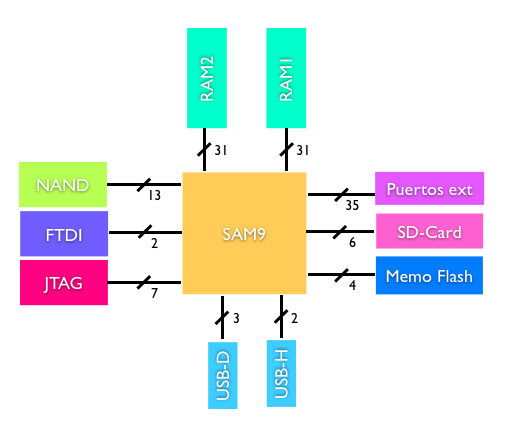
\includegraphics[scale=0.6]{img/diagrama_bloques}

\caption{\label{fig:bloques}Diagrama de bloques de SAM9-MX}



\end{figure}


\pagebreak{}


\subsection{Diagrama Esquem\'atico}

La elaboración de un diagrama esquemático no es tarea fácil, sobre
todo tratándose de un dispositivo tan grande y complejo como lo es
la SAM9-MX, es por eso que en esta sección se explicarán los pasos
que seguimos para tener un diagrama esquemático listo.

El diagrama esquem\'{a}tico es una representaci\'{o}n pict\'{o}rica
de un circuito el\'{e}ctrico. Muestra los diferentes componentes del
circuito de manera simple y con pictogramas uniformes de acuerdo a
normas y las conexiones de poder y de señales entre los dispositivos.
El arreglo de los componentes e interconexiones en el esquema generalmente
no corresponde a las ubicaciones físicas en el dispositivo terminado. 

Si bien una tarea más difícil es la elaboración del PCB, se tiene
que tener en mente, las medidas de los diferentes componentes que
integran esta tarjeta, para así poder asignar footprints adecuados
y hacer el camino del PCB más sencillo.

Para hacer el diagrama esquemático se probaron varios software especializados
en ese campo, automatizar el diseño de circuitos electrónicos. Los
cuales fueron:
\begin{enumerate}
\item gEDA
\item Orcad
\item Eagle
\end{enumerate}
Cuando se utilizó gEDA, se pudieron realizar varios diagramas pruebas,
pero no era tan fácil de usar para hacer los footprints de los componentes,
así que se decidió seguir con la investigación de otros programas
de diseño.

Orcad es un programa más usado para diseñar estos tipos de diagramas,
por lo mismo se empezó a usar y a hacer diferentes diagramas prueba
junto con sus respectivos PCB's, pero a la hora de investigar los
tamaños y medidas exactas de los diferentes componentes, se pudo observar
que ya existían bibliotecas con los footprints de cada uno para un
programa llamado Eagle.

Eagle, es el programa que se esta utilizando en este momento, se utilizó
para el diagrama esquemático y posteriormente con el se hará el PCB,
el hecho de que encontráramos a los componentes en las diversas bibliotecas
distribuidas en internet, fue de gran ayuda, para la elaboración del
diagrama.

\pagebreak{}


\subsubsection*{Microcontrolador}

Ya que se tiene el programa que se va a usar y se verifican que las
partes del diagrama se encuentren; en nuestro caso se puso primero
el microcontrolador pues es el que más pines tiene y el que esta conectado
a casi todos los componentes de la \ac{SAM}9-MX.


\subsubsection*{Memorias}

Después del micro se pusieron las memorias, pues son de gran importancia
para nuestra tarjeta, contamos con dos memorias RAM las MT48LC64MA2,
cada una cuenta con 12 pines de direcciones y 15 pines de datos que
estan conectados al micro. Los pines de direccion se conectan al los
mismos puertos en el micro, sin embargo los datos esta conectados
a puertos distintos, esto es por que cuando queremos hacer un acceso
a memoria, los pines de direccion nos regresan la dirección de la
misma, pero una RAM nos regresa la parte alta de los datos, mientras
que la otra nos regresa la parte baja. 

Así mismo, también se cuenta con una memoria NAND, la cual se puede
deshabilitar por medio de una jumper, y con eso se habilitan las memorias
RAM, esto es de gran ayuda a la hora de programa la tarjeta pues no
se puede programa con la NAND habilitada. La memoria NAND comparte
la sección de datos del microcontrolado con una RAM.

En cuento memorias faltaría una de citar, la memoria FLASH, que cumple
la función de cualquier otra memoria FLASH, hacer el acceso a memoria
más rápido. Claro esta, esta es de menor capacidad que las demás pero
ayuda mucho a agilizar los accesos, por lo tanto cumple su función
y el objetivo de ser puesta en la tarjeta.

Otro dispositivo importante es la memoria SD Card, escogimos que fuera
una micro SD por que es un componentes novedoso, de fácil uso y sirve
para almacenar datos que pueden posteriormente ser guardados en la
tarjeta.

\pagebreak{}


\subsubsection*{Alimentaci\'on}

La alimentaci\'{o}n de la tarjeta, es donde se obtiene el voltaje
que se necesita para alimentar a todos los componentes de la tarjeta
los cuales en su mayoría operan con 3.3V. 


\subsubsection*{Puertos}

Puertos usb: cuenta con dos, uno de ellos es un puerto USB Device
el cual se puede comunicar con la computadora por medio un cable USB,
y el otro puerto USB es Host, lo que nos permite directamente conectar
nuestra memoria USB a la tarjeta, estas son unas funciones innovadoras
y fáciles de usar para el empleo de nuestra tarjeta. 

Otro componente importante es el JTAG, el cual nos sirve para programar
y debuggear nuestra tarjeta, tambi\'{e}n nos ayuda a saber los estados
de los registros de la memoria, cuando se est\'{a} en tiempo de ejecuci\'{o}n.

Los puertos externos, previniendo que en un futuro se quieran conectar
m\'{a}s componentes de los que tiene esta tarjeta, se pueden hacer
en este espacio, que va directamente relacionado con los puertos B
y C del micro. Ya que este es uno de los principales objetivos de
nuestro trabajo terminal, la propiedad de expansión, para que futuras
generaciones puedan hacer innovaciones con ellas. 


\subsubsection*{FTDI}

Antes de este diagrama, el esquemático de la \ac{SAM}9-MX, se efectuó
el diagrama del dispositivo FTDI, ya que es más simple que el de la
\ac{SAM}9-MX; sirvió para probar los diferentes programas para realizar
diagramas, el FTDI nos permitirá tener una comunicación con la tarjeta
desde nuestra computadora por medio de un USB, en lugar de con otros
puertos que muchas de nuestras portátiles ya no cuentan.

El diagrama esquemático de la \ac{SAM}9-MX dividido en 4 partes,
junto con el diagrama del FTDI, se encuentran en el apéndice y\ref{ch:esquematico}.

\section{Desarrollo}

Desarrollar un circuito impreso es una tarea muy complicada, detallada y tardada, se necesitan en realidad muchas horas y mucha paciencia para poner todos los componentes en su lugar o en el mejor lugar posible.

\subsection{De diagrama esquemático a PCB}

Para pasar de diagrama esquemático a PCB

\begin{enumerate}
\item Revisar que no falte ningún componente.
\item Invocar todos los pines de todos los componentes.
\item Tener cuidado con los diferentes paquetes.
\item Correcta conexión entre todas las líneas ruteadas. 
\item Revisar nodos.
\end{enumerate}

Cada uno de los puntos anteriores se deben hacer con especial dedicación, para poder pasar al desarrollo del PCB un poco más confiados.

\subsection{Pasos a para hacer un PCB}

Se recomienda seguir una series de pasos y sugerencias que se pueden llevar a cabo en la elaboración de un PCB, que hace el desarrollo si bien no tanto más rápido, más entendible y limpio.

Los pasos para desarrollar el PCB, son los siguientes:
\begin{enumerate}
\item Establecer la medida de la tarjeta.
\item Poner los componentes dentro de la tarjeta.
\item Ordenar los componentes.
\item Hacer las interconexiones.
\item Checar ángulos de las conexiones.
\item Revisar ruido y campos magnéticos.
\item Revisar consistencia con el diagrama esquemático.
\end{enumerate}

\subsubsection*{Establecer las dimensiones de la tarjeta.}

Siempre es bueno tener en mente el tamaño que queremos que sea nuestra tarjeta aunque muchas veces la cantidad de componentes que tiene, nos dificulta poner una medida fija, se debe de tener una estimación.

En nuestro caso la tarjeta es 16 cm por 10 de ancho. Lo cual es un tamaño aceptable para aún dispositivo que se pensó fuera portátil.

Se hicieron varias versiones de la tarjeta, algunas eran más chicas y los componentes cuando se tenían que acomodar dentro, quedaban muy juntos, otras fueron más grandes y sobraba mucho espacio. Así que cuando se llego a este tamaño fue el ideal con el acomodo de componentes.

\subsubsection*{Poner los componentes dentro de la tarjeta.}

Este paso es de ayuda para determinar el tamaño de la tarjeta por qué aunque no es el lugar definitivo de cada componente se tiene que poner una estimación aproximada de los mismos. 

\subsubsection*{Ordenar los componentes.}

Para ordenar los componentes se debe de tomar en cuenta algunos puntos que son un estándar, que hace que la tarjeta se vea mejor.

\begin{itemize}
\item Los componentes deben de ser alineados de manera que estén organizados con espacio uniforme.
\item Los componentes deben estar orientados de manera que las esquinas deban ser paralelas a la esquina de la tarjeta.
\item Si la tarjeta es soldada por máquina, se recomienda que los componentes que atraviesan la placa se pongan de un solo lado de la tarjeta, mientras sea posible.
\item Cuando se ponen los componentes en ambos lados de la tarjeta y se mezclan componentes de montaje superficial con algunos que no, se debe de tomar en cuenta que se necesiten muchas capas lo cual genera aumento de costos y mayor riesgo de fallos.
\item No es recomendable poner componentes de plomo o de titanio en la parte baja de la tarjeta.
\item Una cuadrícula 2.5 mm debe de ser usada, sin embargo es posible usar una de 0.5 mm o inclusive 0.05 si se requiere por componentes no estándar
\item Para diseños que van a ser probados en una "cama de clavos", se debe de usar una cuadrícula de 2.54 mm
\item Los diodos y capacitores polarizados deberán de ser alineados consistentemente a lo largo de toda la tarjeta, para facilidad de inspección y pruebas.
\item Si el diseño lo permite se deberían de poner los conectores en en el lado corto del diseño.
\item Distribuir el espacio en el montaje de los componentes para permitir el montaje del hardware.
\item Los componentes que pesen más de 0.5g deberán de tener soporte mecánico en caso de que la tarjeta experimente vibración.
\item El manejo del calor debe de ser tomado en cuenta para el diseño del circuito.
\item Las consideraciones eléctricas tienen prioridad sobre las consideraciones mecánicas cuando hay conflicto entre las dos exceptuando el hecho de que se llegue a una falla mecánica en el diseño.
\item Para señales mixtas (analógica, digital) los componentes deberán de estar segregados para minimizar el efecto del las señales analógicas en la tarjeta.
\end{itemize}

\begin{figure}
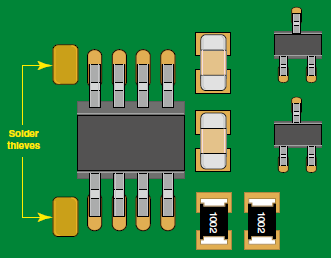
\includegraphics[scale=0.6,angle=0]{img/OrdenComponentes.png}\caption{Ejemplo de componentes ordenados}
\label{Flo:OrdenComponentes}
\end{figure}

\ref{Flo:OrdenComponentes}
Es importante recalcar que los pasos anteriores son recomendaciones y que muchas veces cuando la tarjeta es grande y/o los componentes son demasiados no se pueden seguir todas.

\subsubsection*{Hacer las interconexiones}

Una vez que ya se tiene la distribución de los componentes y el tamaño de la tarjeta, ya el siguiente paso es el ruteo. La manera más fácil es dejar que el programa rutee la tarjeta por nosotros, pero no siempre puede hacerlo al 100% muchas veces se queda al 70%, se puede escoger cuantas veces quiere que se vuelva a intentar seguir ruteando la tarjeta o que vaya optimizando los caminos, de cualquier manera la ayuda que hace el sistema nos facilita un poco más el trabajo y nos ahorra un poco de tiempo.

Cuando se tiene que rutear manualmente se debe de ser muy cuidadoso, los principales puntos que hay que tomar en cuenta son que:

\begin{itemize}
\item{Cruces de las lineas de ruteo de una misma capa}
Algunas veces las lineas de la misma capa se cruzan entre sí ocasionando errores pues eran puntos que no se debían tocar, por lo mismo se debe de tener mucho cuidado a la hora de rutear de revisar todas las lineas por las que se esta pasando. Por que a veces pudiera parecer que no están juntas las lineas pero la proximidad ya en la tarjeta física ocasionaría muchos errores.

\item{Cambios de capa}
Cuando ya no se puede llegar a un camino con una linea de una misma capa se debe de hacer un cambio de capa, al hacerlo se debe revisar que los cambios se realicen de manera correcta, no habiendo separaciones que podrían traducirse como pérdida de continuidad.

\item{Grosor de las lineas}
El tamaño de grueso de las lineas también debe ser acorde a las proporciones de la tarjeta. 

La mayoría de las tarjetas de productos comerciales hoy en día son de tamaños muy pequeños con componentes diminutos y pistas igual de pequeñas en grosor. 

Por esa razón, siguiendo al patrón se realizaron pistas delgadas, que guardaran su distancia con las demás pistas de la tarjeta pero que pudieran ser de un tamaño adecuado para que quepan todas en un espacio reducido

\item{Sentido de las lineas}
Esta tarea es muy tardada y se necesita de mucha concentración.

Para rutear a la SAM9-MX se necesito primero establecer dos capas en las que el programa intentara rutear la tarjeta. Después se configuro una capa tercera para los ruteos manuales. Ahora se procedía a tomar una línea que estuviera todavía sin rutear y se escogía la capa en la que se quería que estuviera. Para esto se seguía otro orden:

La capa superior, la roja, se movía mayormente de manera vertical.
La capa inferior, la azul, iba de manera horizontal.
La capa que cruza por en medio, azul con rayas, la mayoría de las veces iba de manera horizontal.

Este fue un paso muy tardado por la cantidad de conexiones que tiene el microcontrolador con los demás dispositivos de la tarjeta. 
\end{itemize}

\subsubsection*{Checar \'angulos de las conexiones.}

Como todas las recomendaciones que se han visto hasta el momento, también se encuentra una recomendación que mas que nada debería ser ley a cerca de las esquinas de las pistas de ruteo.

Se dice que las esquinas no pueden terminar en ángulo recto pues eso hace que cueste más trabajo y tiempo para que las señales se transmitan pues deben de hacer todo un giro de 90º,

Por lo tanto cuando se va ruteando es recomendable ir haciendo diseños que sean ortogonales de las esquinas y si ya se acabo el diagrama. Se debe de revisar parte por parte como quedan las pistas, para corregir aquellas que se puedan, las cuales siempre se esperan sean la mayor cantidad posible.

\subsubsection*{Revisar ruido y campos magn\'eticos.}

Dependiendo de la calidad y forma de la tarjeta se deben de tomar algunas consideraciones para el diseño de la misma, por ejemplo, se debe de revisar que no se tenga ruido, o que los campos magnéticos no generen algún problema a la tarjeta.


\subsubsection*{Revisar consistencia con el diagrama esquemático.}

Un punto muy importante que no se debe de dejar para el último es revisar la consistencia entre los diagramas, pues a veces sin desearlo se hacen algunos cambios de los que no se da uno cuenta hasta que el diagrama esquemático manda muchas advertencias. 

\subsection{Diseño final del sistema m\'inimo.}

Esta es la tarjeta SAM9-MX 2 ya realizada en un PCB lista para la posterior fabricación de la misma.

\subsubsection*{Caracter\'isticas de la SAM9-MX}

\begin{itemize}
\item Aproximadamente 150 dispositivos (entre resistencias, capacitores, puertos, memorias...)
\item Microcontrolador de 208 pines.
\item Memorias Ram de 54 pines.
\item Dimensiones de la tarjeta : 16 x 10 cm, Grosor 5mm
\item 3 capas de ruteo.
\item Aproximadamente 400 lineas de ruteo.
\item Porcentaje de ruteo : 69.8% automáticamente y 30.2 % manual.
\item Ancho de lineas : 0.01m.
\item Sexta versión.
\end{itemize}

El diagrama de la SAM9-MX con todos sus componentes se presenta en el apéndice
\ref{ch:esquematico}.

\subsection{Factibilidad de realizar la SAM9-MX impresa}

Una de las decisiones importantes que se tomó ya en el proceso de desarrollo de este trabajo fue la de realizar un simulador de la SAM9-MX llamado ARMyC en lugar de realizar la tarjeta hasta su terminación.

Se tuvieron dos grandes consideraciones par esta decisión: la primera era la falta del tiempo y la segunda que los costos de fabricación en total habían incrementado considerablemente. Así que mucho antes de que fuera demasiado tarde se realizó un estudio de factibilidad de la fabricación la tarjeta. 

El estudio se realizo con empresas extranjeras de origen asiático específicamente pues estas son las que tienen el producto en un menor tiempo de espera a un menor costo y con la calidad que se requiere.

De una forma más desglosada los factores que se consideraron se enlistarán a continuación:

\begin{itemize}
\item Costo de fabricación de la tarjeta.
\item Costo de envió de la tarjeta.
\item Tiempo de envió de la tarjeta.
\item Tiempo de fabricación de la tarjeta
\item Costo de los restantes componentes
\item Tiempo de espera por los demás componentes
\item Tiempo de soldado de los componentes
\item Tiempo de pruebas de la tarjeta
\end{itemize}

Ahora, se debe de tomar en cuenta que hacer una sola placa de las características de nuestra tarjeta resulta muy costosa, pues a ninguna empresa especializada le conviene realizar una sola tarjeta. 

Por eso, normalmente los pedidos son de 100 ó 1000 placas a imprimir pero nosotros imprimiríamos la cantidad de cuatro, en promedio el costo de las 4 placas es de 700 USD. Si fueran en mayores cantidades el precio disminuiría considerablemente, pero no necesitamos 96 placas más.

El costo de envió es aproximadamente de 50 USD, debido a la lejanía entre el país de fabricación y México.

El tiempo de entrega de la placa sería de 8 semanas pues se considera el tiempo de fabricación más el envió, este último es más tardado que el anterior.

Aparte, no se tienen aún todos los componentes de la SAM9-MX, faltan algunas memorias y demás dispositivos esenciales que se deben de mandar a pedir de igual manera a un país extranjero en este caso Estados Unidos es el que nos queda más cerca  comprar la totalidad de los componentes, costaría aproximadamente 500 USD.

El tiempo de espera de los componentes es de 2 semanas aproximadamente. El costo de envió de los componentes es de 30 USD. Si bien este paso se puede hacer en paralelo con el paso de mandar a pedir la tarjeta, es mucho más el tiempo que se tiene que esperar para entrega de la tarjeta.

Una vez que ya que se tienen las tarjetas junto con todos los componentes se procede a soldar estos últimos a la tarjeta. El soldado de la totalidad de los 150 componentes es de aproximadamente 2 semanas pues es una tarea muy exacta que se debe de realizar con mucha dedicación y paciencia.

Se necesita probar todos los puertos y dispositivos para esto se tiene que hacer de todas maneras un simulador y verificar el correcto funcionamiento de la tarjeta en manera general y de los dispositivos específicos. Finalmente, este proceso sería aproximadamente de 2 semanas.

Así que haciendo un cuadro de actividades, tiempo y costos quedaría así.

\begin{figure}
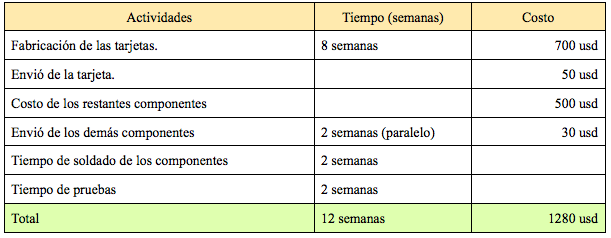
\includegraphics[scale=0.6,angle=0]{img/cuadroPCB.png}\caption{Cuadro que representa el estudio de factibilidad del PCB}
\label{Flo:cuadroPCB}
\end{figure}

Este era uno de los mejores escenarios a evaluar, de hecho era el promedio en cuanto a las empresas que investigamos, algunas actividades podrían disminuir en tiempo, pero aumentarían en costo.

Por esas dos razones se optó por la propuesta de realizar un simulador, que su nombre lo dice, haga la representación de los componentes de la tarjeta, como si esta estuviera impresa.

\subsection{Gerber files}


